\newcommand{\Koord}{\ensuremath{\lgname}\xspace}
\newcommand{\CyPhyHouse}{CyPhyHouse\xspace}
\newcommand{\Gazebo}{Gazebo\xspace}

\newcommand{\ScanToMap}{\ensuremath{\mathit{scanToMap}}\xspace}
\newcommand{\TSync}{\ensuremath{\mathit{tSync}}\xspace}
\newcommand{\PathToFrontier}{\ensuremath{\mathit{pickPathToFrontier}}\xspace}

\section{Case study: Distributed Mapping application}
\label{sec:experiments}

For our case study, we test the \dmap application using the simulator from \CyPhyHouse~\cite{ghosh2019cyphyhouse} for distributed \Koord applications.
We choose the MIT RACECAR model~\cite{MIT_RACECAR} with Lidar sensor included in \CyPhyHouse for our experiment.
To implement external functions defined in~\ref{sec:analysis},
we extend the \CyPhyHouse tool chain and examine our assumptions over sensor data and implemented functions.
In the section, we first discuss our implementation of external functions;
then we present the simulation result of \dmap with multiple vehicles.


\subsection{Implementation of External Functions}

\paragraph{Sound Mapping from Synchronized Sensor Data~(\ScanToMap).}
To generate a 2D map from the scan data,
it is required to synchronize the current vehicle position and the Lidar scan data~(\TSync).
An existing solution is to filter the time stamps of both sensor data streams
and only choose pairs of data within a given time difference threshold $\epsilon$.
This can be achieved by \texttt{ApproximateTimeSynchronizer} in the ROS package named \texttt{message\_filter}.
The frequency of the synchronized data is then limited to the sensor with the lowest frequency.
In our simulation, the lowest frequency is 100 Hz for sensing the vehicle position and sufficient for updating the map.

The Lidar scan data provided in the tool chain are pairs of a distance to obstacles and an angle with respect to the heading angle of the vehicle.
To implement \ScanToMap, it is then straightforward to compute the positions of obstacles and mark occupied grid rectangles,
and to mark a rectangle obstacle free is to simply check if all four corners of a grid rectangle are covered in the scan.
The time difference $\epsilon$ however can introduce an error between real and perceived distances to obstacles.
Reducing this error is beyond the scope of this work.
Our implementation of \ScanToMap therefore may falsely mark a grid rectangle as occupied when obstacles are in nearby grids.

\paragraph{Path to Frontier~(\PathToFrontier).}
In the \CyPhyHouse tool chain, several path planning algorithms are already available.
We particularly select the Rapidly exploring Random Tree with near neighbor search and rewiring tree~(RRT*) algorithm.
It is able to avoid obstacles and is fine tuned to the car model for simulation.
Our \PathToFrontier implementation hence only needs to choose a point in frontier grid rectangles and provide the positions of obstacles.
To choose such a point, a basic solution is to use Breadth-First Search~(BFS) on the map and seek for a unexplored grid rectangle.
BFS ensures that either all reachable grid rectangles are marked,
or there are connected unoccupied rectangles to an unexplored rectangle, and hence a path must exist.
Nonetheless, it does not guarantee that the underlying path planner can always find a path because,
for instance, the car is incapable of make sharp turns.
Our soundness claim still holds under such circumstance, but we may not be able to progress even when paths to frontier exist.


\subsection{Simulation Result}

We design three different worlds with the same area of $20\times20$ square meters,
and each can be quantized as a $20 \times 20$ map.
To compare across different numbers of vehicles more easily,
we ensure that all unoccupied rectangles are connected in each map,
so every car can explore the whole map.
Each car is equipped with a Lidar providing each scan with radius 2.5m and angles from $-\pi$ to $\pi$.
For simplicity, we configure the Lidars so that they do not detect other cars as obstacles.
The maximum speed of all cars is set to 3m/s.
For each map, we run three simulations with 2, 3, or 4 cars for 20 minutes of simulation time.
Our simulation is run on a computer with 8 Intel Core i7-6700HQ @ 2.60GHz CPU cores, 16 GB main memory, and a GeForce GTX 970M GPU.


\begin{figure*}[t]
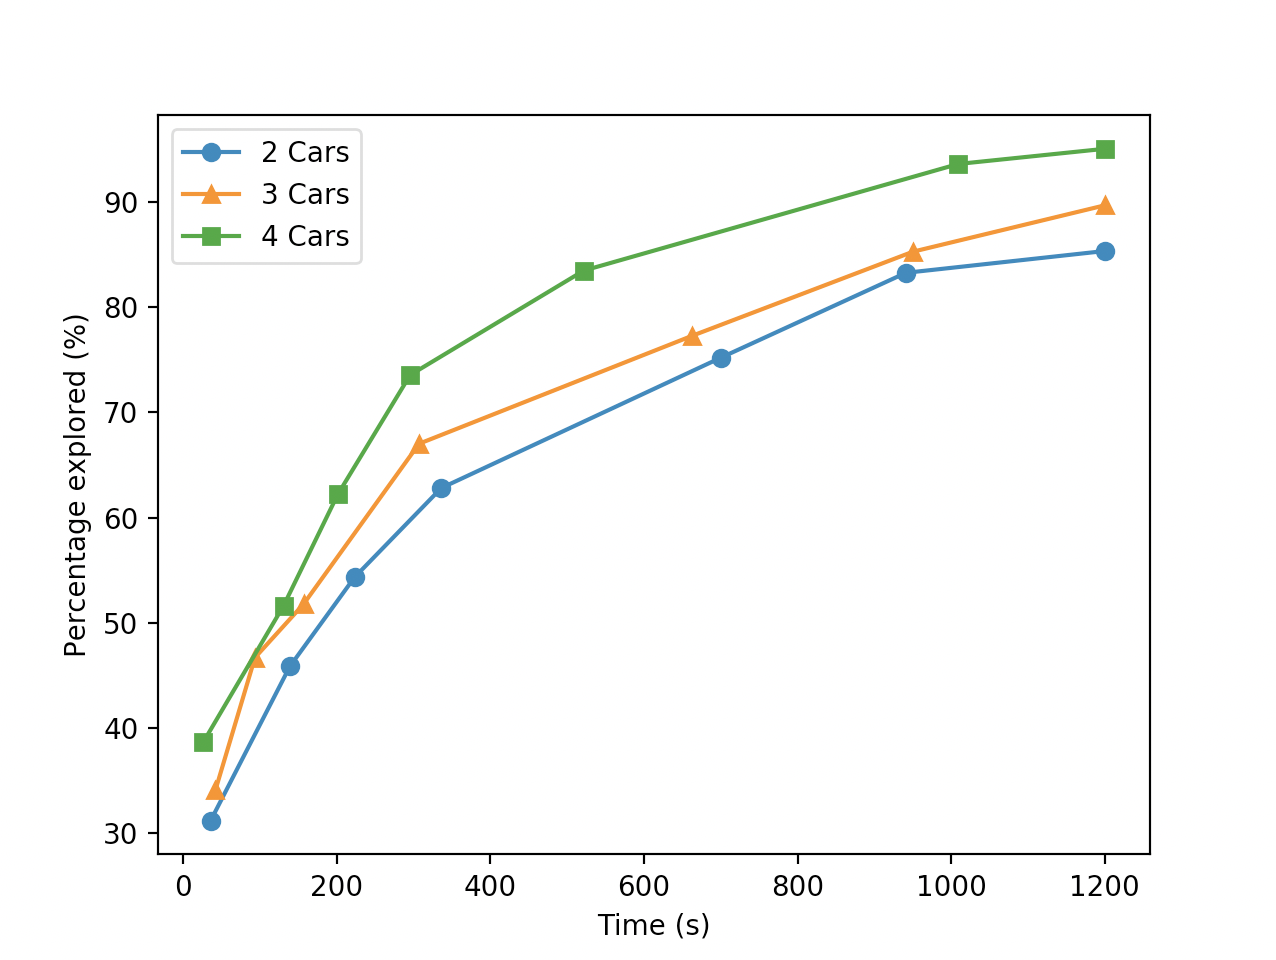
\includegraphics[width=0.3\textwidth]{figs/exp-empty.png}
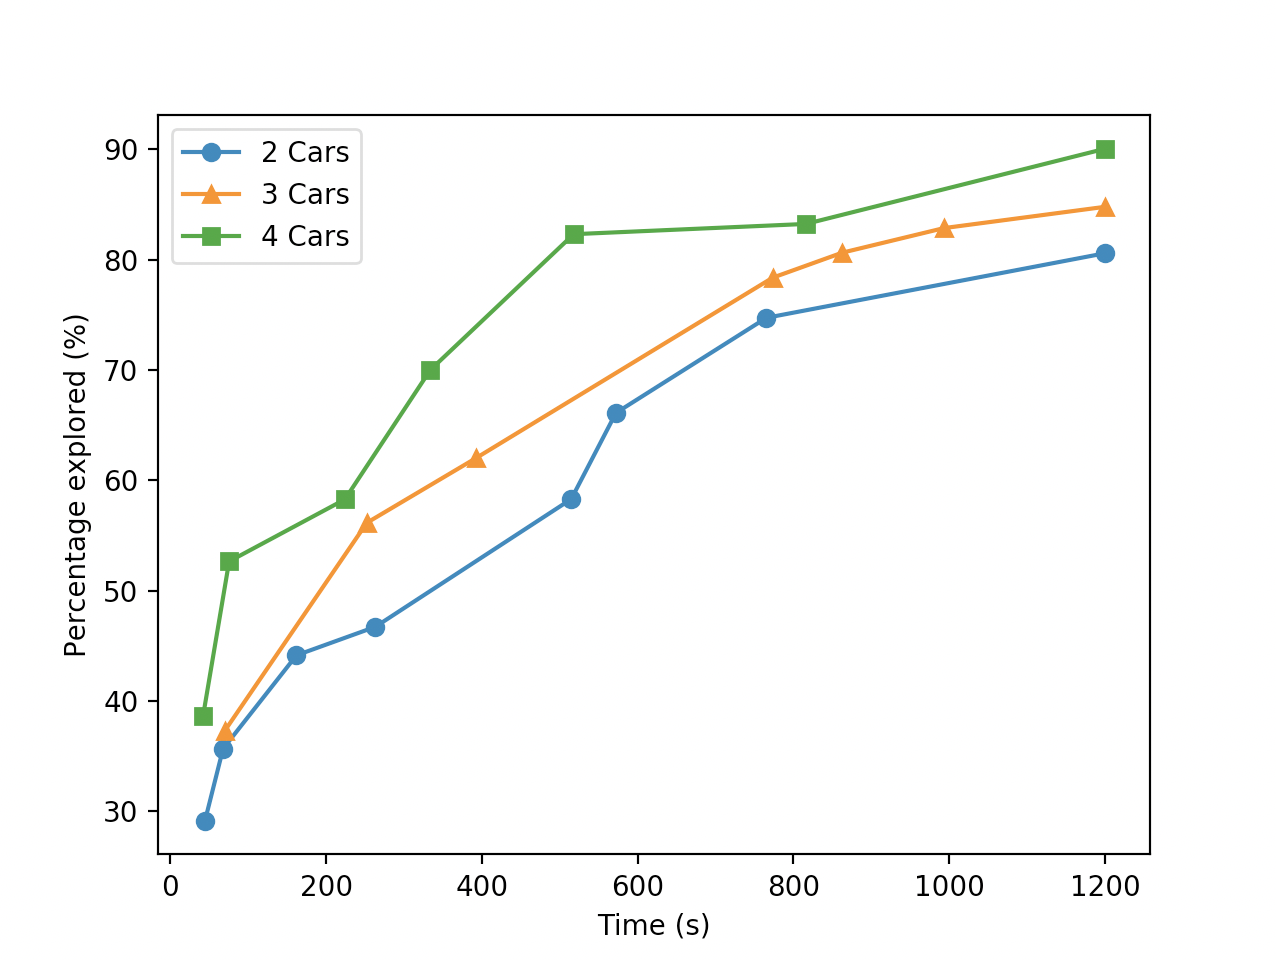
\includegraphics[width=0.3\textwidth]{figs/exp-u-shape.png}
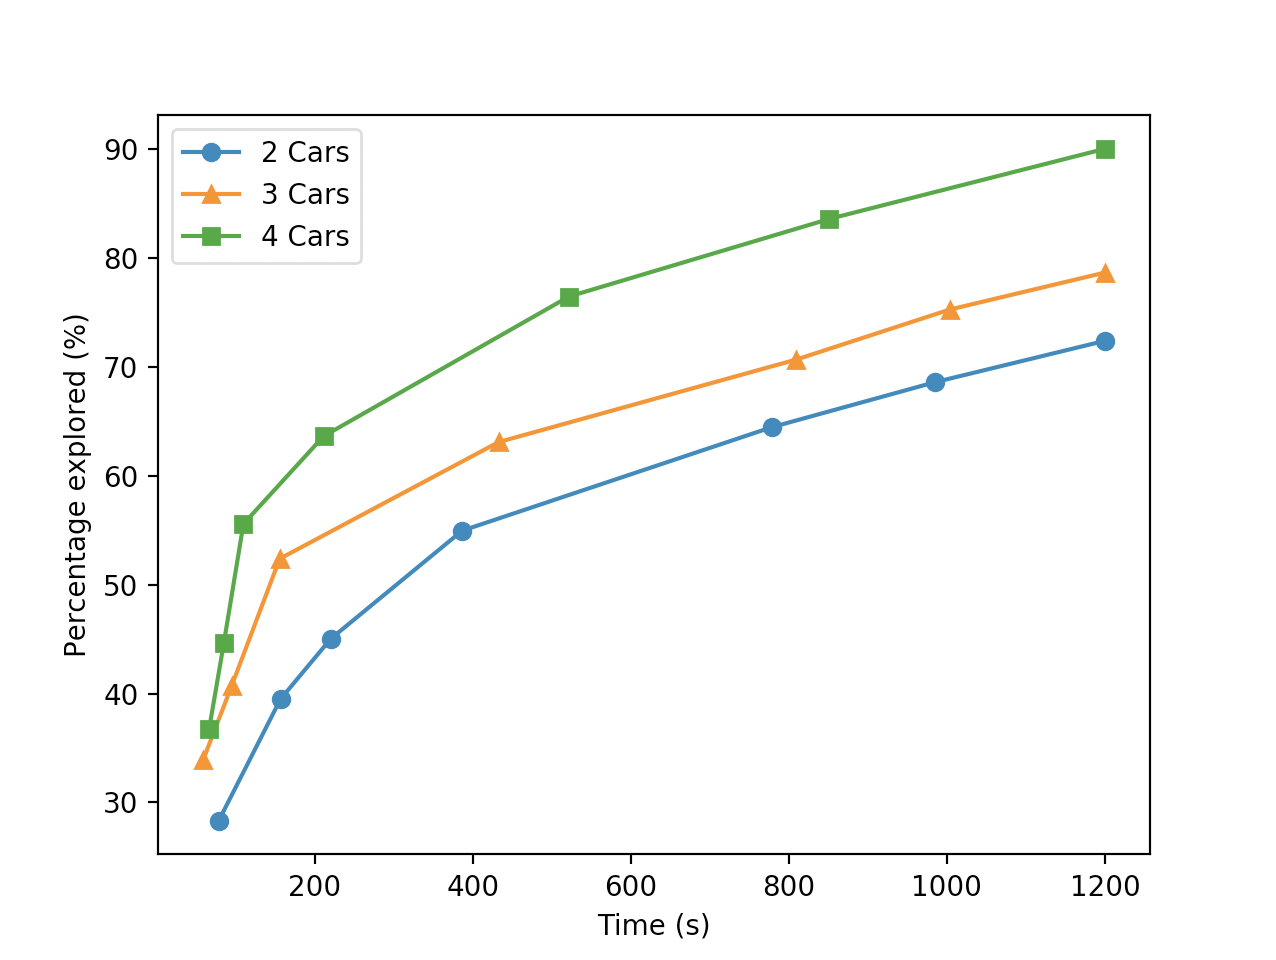
\includegraphics[width=0.3\textwidth]{figs/exp-i-shape.png}
\caption{Percentage of exploration for map without obstacles~(\emph{Left}), with U-shape~(\emph{Mid}), and with I-shape~(\emph{Right}).}\label{fig:percent}
\end{figure*}

\begin{figure*}
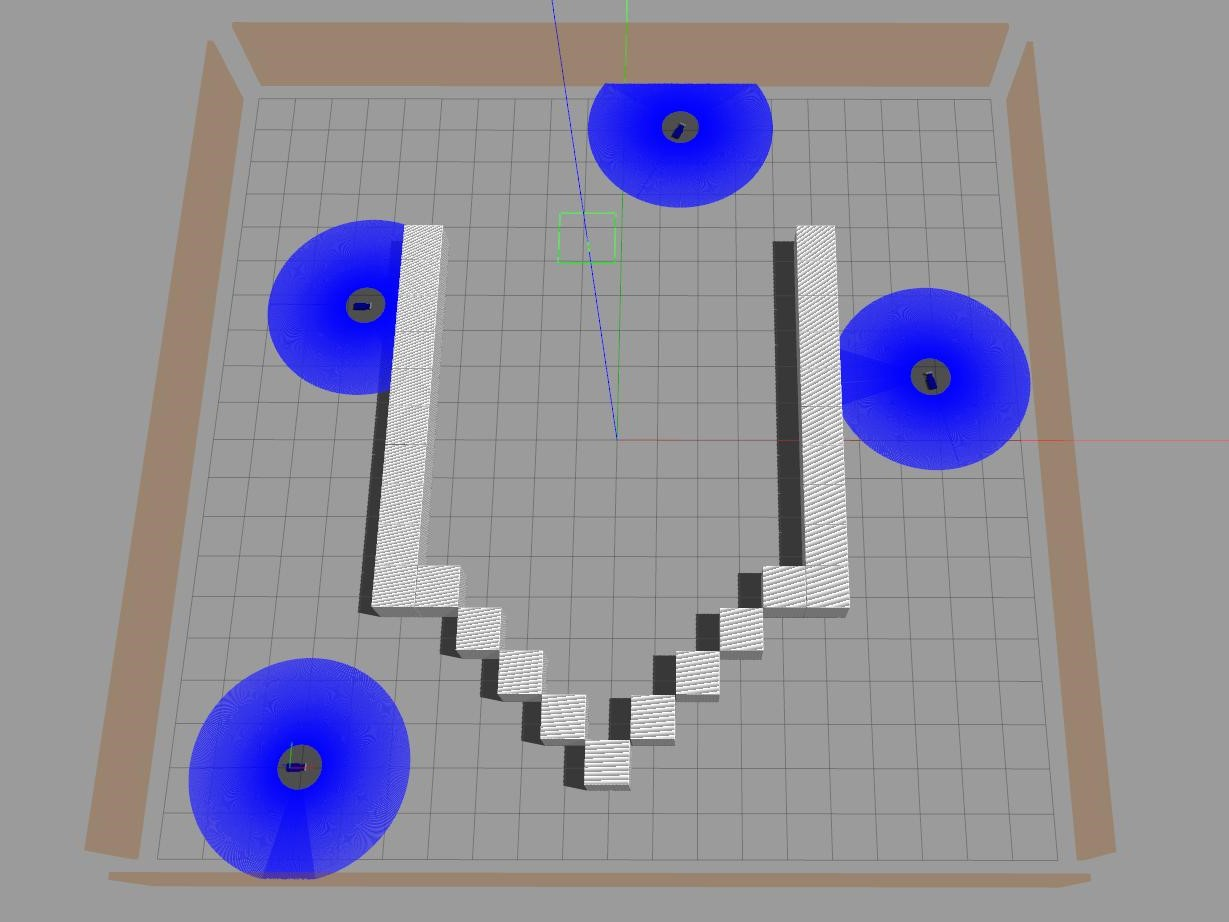
\includegraphics[width=0.3\textwidth]{figs/exp-gazebo.jpg}
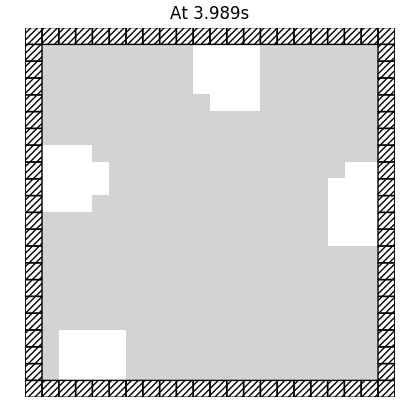
\includegraphics[width=0.22\textwidth]{figs/exp-progress-1.png}
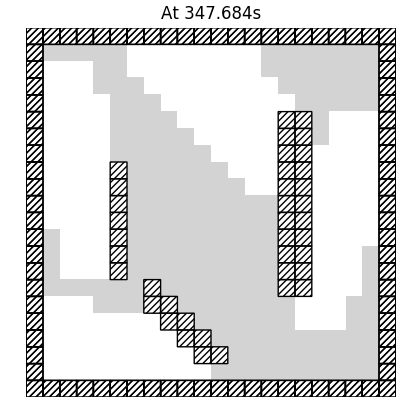
\includegraphics[width=0.22\textwidth]{figs/exp-progress-2.png}
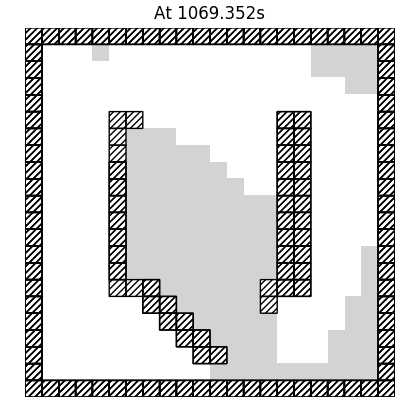
\includegraphics[width=0.22\textwidth]{figs/exp-progress-3.png}
\caption{Four cars in U-shape world in simulator~(\emph{Left}). Visualization of the global map at three different time stamps~(\emph{Right})}\label{fig:U-map-progress}
\end{figure*}

Figure~\ref{fig:percent} shows that more cars explore more percentages in any given amount of time in all maps.
It is not surprising because more cars start with more areas explored initially and explore concurrently.
A more interesting result is that the final saturating percentages by more cars are higher as well.
From our observation in the visualization, one major reason is due to the aforementioned limitations in finding paths to frontier.
When there are only few unexplored grid rectangles remaining,
it becomes much more difficult to find such paths.
The chance to successfully find such path with more cars is simply higher.
The U-shaped obstacle in Figure~\ref{fig:U-map-progress} is designed to demonstrate this problem.
Note that only the car at the top can reach the center of the map without much trouble.
However, we deliberately place it to face the boundary wall.
As a consequence, the center of the map is much less explored.

In short, our experiment shows our \dmap application can be deployed to more devices with little effort.
With more devices, it can explore the map faster and more complete.
We also see that the difficulty to achieve completeness largely depends on the limitations of underlying devices and path planning algorithms.
